\documentclass[kulak]{kulakarticle} % options: kulak (default) or kul

\usepackage[dutch]{babel}
\usepackage{pdfpages}
\usepackage{graphicx}
\usepackage{mathtools}
\usepackage{nccmath}


\title{Smart Fire Extinguisher - Tussentijds Verslag}
\author{TEAM 6: Anna-Laura, Emile, Jérôme, Jesse}
\date{Academiejaar 2022 -- 2023}
\address{
	\textbf{Groep Wetenschap \& Technologie Kulak} \\
	Ingenieurswetenschappen \\
	P\&0 2}

\begin{document}

\maketitle

\section*{Inleiding}

Bij de brandbestrijding in grote warenhuizen worden momenteel sprinklers gebruikt. Deze zijn vastgemaakt aan het plafond van het gebouw en zijn aan de waterleiding aangesloten om bij brand water te doen neerdalen en de brand te blussen. Ze blussen heel efficient branden, maar er zijn ook bepaalde nadelen aan. De aanleg en het onderhoud van alle leidingen die de sprinklers van water voorzien is een hele dure onderneming. Ook kan bij het springen van een van de waterleidingen heel veel water verloren gaan alsook goederen beschadigen. \\

Daarom zijn wij op zoek gegaan naar een efficientere manier om branden te blussen. Een Smart Fire Extinguisher, die zelf de branden kan detecteren, localiseren en gericht kan blussen. Zo zou 1 apparaat (met dus maar 1 aansluiting op de waterleiding of een eigen waterreservoir) een groot oppervlakte brandveilig kunnen maken. Dit zou het veel goedkoper maken voor de eigenaar die geen eindeloos lange waterleidingen moet aanleggen en onderhouden.


\section{Ontwerp}

We opteren voor een stationair brandblusplatform dat gebruik maakt van een draaiend platform en een arm om het water in de juiste richting en onder de juiste hoek weg te spuiten. Water uit een waterreservoir zal dan met behulp van een pomp op de gewenste plaats terecht komen. Deze plaats zal zijn vastgesteld door een camera. Deze detecteert de brand en aan de hand van de beelden zal er berekend worden waar en hoe ver de brand zich bevind ten opzichte van het brandblusplatform. Daarna zullen nog een hoop berekeningen de hoek van de twee armen bepalen. \\

Voor het detecteren van de brand maken we gebruik van een webcam (USB Webcam 1080P), in Python wordt een programma geschreven op een laptop die aan branddetectie en -localisatie doet. Deze is vastgemaakt op het roterend platform. \\

De beweging van het draaiend platform en de arm gebeurt met behulp van twee motoren (Micro Metal Gear Motor 100:1 HP), deze zullen dankzij een motor drive met de gewenste snelheid en in de juiste richting draaien. Volgens de berekeningen gedaan door een laptop en webcam kunnen de armen zich juist positioneren. \\

Als de arm juist gericht staat, is het enige dat overblijft het blussen van de brand. Hiervoor zal de pomp (Membraanpomp 12V 4.8 bar) water uit het waterreservoir (jerrycan 10L) door een slang (met diameter 10mm) pompen, om zo weggespoten te worden richting het doelwit. Het water de benodigde afstand doen kunnen afleggen om het volledige bestrijkingsgebied te kunnen bestrijken is mogelijk door het aanpassen van het mondstuk.


\section{Berekeningen}
\subsection{Water}

De afstand zoals te zien in afbeelding \ref{schematische voorstelling} tussen het brandblusapparaat en de cilinder is \(x\) waarbij \(x\) maximaal gelijk kan zijn aan \(10,45 m\). Om deze afstand te halen berekenen we de hoek waaronder het water moet worden weggespoten. De hoogte van het platform is hier \(h_1\) en de hoogte van de arm is \(h_2 = lsin(\theta)\) met \(l\) de lengte van de arm. \(y\) is de hoogte van de cilinder die moet worden opgevuld. Dan krijgen we:
\begin{equation}
	\begin{cases}
		x  = cos(\theta) v t \\
		y = h_1 + h_2 + sin(\theta) v t + \frac{-1}{2} g t^2
	\end{cases}
\end{equation}
Bij het gebruik van de brandblusser zullen we met behulp van de camera \(x\) al kennen, dankzij de waterflowsensor zullen we \(v\) ook accuraat kennen, \(h_1\) staat vast en \(h_2\) hangt af van de hoek \(\theta\). Uit de twee vergelijkingen kunnen we \(\theta\) en \(t\) halen en zal het doelwit gevuld geraken.
\begin{figure} [h!]
	\centering
	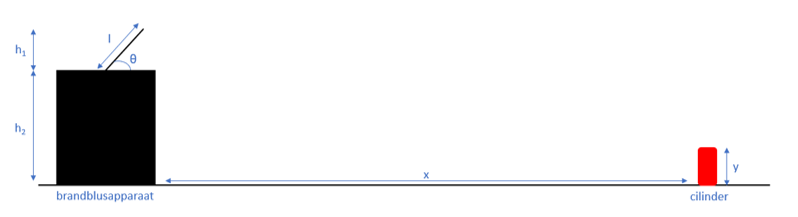
\includegraphics[width = 1 \textwidth]{schematische voorstelling water LATEX}
	\caption{Schematische voorstelling van de opstelling}
	\label{schematische voorstelling}
\end{figure}


\subsection{Camera}
\begin{figure} [h!]
	\centering
	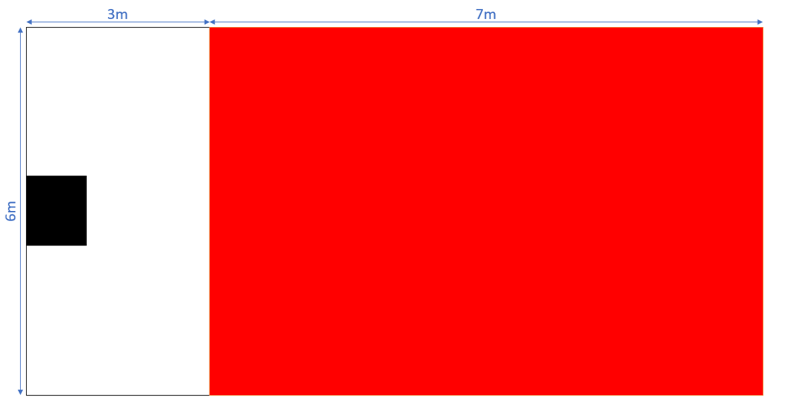
\includegraphics[width = .75 \textwidth]{schematische voorstelling bestrijkingsgebied LATEX}
	\caption{Schematische voorstelling van het bestrijkingsgebied}
	\label{bestrijkingsgebied}
\end{figure}
Omdat het gezichtsveld van de camera niet het volledige bestrijkingsgebied omvat, hebben we besloten de camera te laten meedraaien met het draaiende platform. 

\subsection{Armen}



\section{Planning}


\section{Vooruitgang}


\section*{Besluit}

Afsluitende tekst.

\end{document}
